\documentclass{article}
\usepackage{verbatim}
\usepackage{fullpage}
\usepackage{amsmath}
\usepackage{graphicx}
\usepackage{subcaption}
\usepackage{listings}
\usepackage{placeins} % for \FloatBarrier
%% package for contiued float
\usepackage{caption}
\usepackage[english,greek, main=greek]{babel}
\usepackage[utf8]{inputenc}
\useshorthands{;}
\defineshorthand{;}{?}

\usepackage{pythonhighlight}

\usepackage[explicit]{titlesec} % number after section name
%% the following lines are used to reset the section counter
%% after 'part' is encountered.
\makeatletter
\@addtoreset{section}{part}
\makeatother
%% the following lines are used to add the section number
%% after the section name
\titleformat{\section}
  {\normalfont\large\bfseries}
  {}
  {0em}
  {#1\ \thesection}
%% number after subsection name
\titleformat{\subsection}
  {\normalfont\large\bfseries}
  {}
  {0em}
  {#1\ \thesubsection}
%% avoid numbering contents
\titleformat{\section}
  {\normalfont\Large\bfseries}
  {}
  {0em}
  {\ifnum\value{section}=0\relax #1\else #1\ \thesection\fi}
\newcommand{\eng}[1]{\foreignlanguage{english}{#1}} % shortcut for inserting english into greek text


\title{
    \includegraphics[width=\textwidth]{~/Pictures/emp.png} \\
    \vskip 5cm
    Νευροασαφής Έλεγχος και Εφαρμογές\\
    \large Άσκηση 2η
    \vskip 5cm
}

\author{Αναστάσιος Στέφανος Αναγνώστου\\
        03119051}

\begin{document}

\maketitle
\newpage
\tableofcontents
\newpage

\section{Θέμα}

Ο κώδικας που χρησιμοποιήθηκε για την εκτέλεση της άσκησης φαίνεται παρακάτω:

\selectlanguage{english}
\begin{lstlisting}[language=Matlab]
% Load data
run('el_load.m')
run('deseasonalization.m')
y = el_lo_des';
n = length(y);
train = round(0.7*n);
rest = round(0.3*n);
% Split data into training and validation sets
trainData = y(1:train); % 70% for training
valData = y(train+1:end); % 30% for validation

% Determine the order of the AR model using cross-validation
maxorder = 20;
cvError = zeros(1, maxorder);
for p = 1:maxorder % Test AR orders from 1 to maxorder
    % Fit AR model of order p
    model = ar(trainData, p);
    % Predict on validation data
    predictions = forecast(model, trainData, rest);
    % Calculate error
    cvError(p) = immse(predictions, valData);
end

% Choose the order with the minimum cross-validation error
[~, optimalP] = min(cvError);

% Estimate AR model parameters using the entire dataset
finalModel = ar(y, optimalP);
\end{lstlisting}
\selectlanguage{greek}

\clearpage
\section{Θέμα}

\selectlanguage{english}
\begin{lstlisting}[language=Matlab]
% Generate the data
n = 100; % number of measurements
p = 80; % dimension of x
x = randn(n, p); % xs from a standard normal distribution
c = [rand(10, 1); zeros(60, 1); rand(10, 1)]; % c with 20 non-zero elements
e = randn(n, 1) * 0.5; % e_i uniformly distributed normal random variables
y = x * c + e; % y_i

% Ordinary Least Squares Estimation
c_ols = (x' * x) \ (x' * y);

% Display OLS estimate
disp('OLS Estimate of c:');
disp(c_ols');

% Lasso Regression with Cross-Validation
[c_lasso, FitInfo] = lasso(x, y, 'CV', 10); % 10-fold cross-validation

% Choosing the best lambda
lambda_optimal = FitInfo.Lambda1SE;
c_lasso_optimal = c_lasso(:, FitInfo.Index1SE);
disp('Optimal Lambda:');
disp(lambda_optimal);
disp('Lasso Estimate with Optimal Lambda:');
disp(c_lasso_optimal);
\end{lstlisting}
\selectlanguage{greek}

\clearpage
\section{Θέμα}

\subsection{Ερώτημα}

Αρχικά ορίζεται μια συνάρτηση που εκφράζει την δυναμική του συστήματος.

\selectlanguage{english}
\begin{python}
import numpy as np
import matplotlib.pyplot as plt

# System dynamics of the pendulum
def pendulum_dynamics(x, a1, a2, b, u):
    x1, x2 = x
    x1_dot = x2
    x2_dot = -a1 * np.sin(x1) - a2 * x2 + b * u
    return np.array([x1_dot, x2_dot])
\end{python}
\selectlanguage{greek}

Ο κώδικας για την ενημέρωση των παραμέτρων είναι:

\selectlanguage{english}
\begin{python}
# Gradient descent update
def update_parameters(x, x_hat, a1, a2, b, u, learning_rate):
    x1, x2 = x
    x1_hat, x2_hat = x_hat

    # Compute the gradients
    e1 = x1 - x1_hat
    e2 = x2 - x2_hat

    # Update rules
    a1_grad = -e2 * np.sin(x1_hat)
    a2_grad = -e2 * x2_hat
    b_grad = e2 * u

    a1 += learning_rate * a1_grad
    a2 += learning_rate * a2_grad
    b += learning_rate * b_grad

    return a1, a2, b
\end{python}
\selectlanguage{greek}

\subsection{Ερώτημα}

Παρατίθεται επίσης ο κώδικας για την προσομοίωση. Το πρώτο κομμάτι είναι προσομοίωση
σε σταθερή είσοδο ενώ το δεύτερο προσομοίωση σε ημιτονοειδή είσοδο.

\selectlanguage{english}
\begin{python}
# Simulation parameters
dt = 0.01  # time step
T = 10     # total time of simulation
t = np.arange(0, T, dt)

# Initial conditions and true parameters
x0 = [np.pi/4, 0]  # initial state
true_a1, true_a2, true_b = 1.0, 0.5, 0.3  # true parameters of the system

# Initial guesses for the parameters
a1, a2, b = 0.5, 0.25, 0.15  # initial guesses

# Learning rate for the gradient descent
learning_rate = 0.01

# Storage for data
x_storage = np.zeros((len(t), 2))
x_hat_storage = np.zeros((len(t), 2))
a1_storage = np.zeros(len(t))
a2_storage = np.zeros(len(t))
b_storage = np.zeros(len(t))

# Initial state
x = np.array(x0)
x_hat = np.array(x0)  # initial estimate

# Simulation loop
for i in range(len(t)):
    # Assuming a constant input u
    u = 1.0

    # System dynamics
    x_dot = pendulum_dynamics(x, true_a1, true_a2, true_b, u)
    x = x + x_dot * dt

    # Estimated dynamics
    x_hat_dot = pendulum_dynamics(x_hat, a1, a2, b, u)
    x_hat = x_hat + x_hat_dot * dt

    # Parameter update
    a1, a2, b = update_parameters(x, x_hat, a1, a2, b, u, learning_rate)

    # Store data
    x_storage[i] = x
    x_hat_storage[i] = x_hat
    a1_storage[i] = a1
    a2_storage[i] = a2
    b_storage[i] = b
\end{python}
\selectlanguage{greek}

\selectlanguage{english}
\begin{python}
# Function to generate a sinusoidal wave
def sinusoidal_wave(t, amplitude, frequency):
    return amplitude * np.sin(2 * np.pi * frequency * t)

# Simulation parameters for sinusoidal wave input
sin_frequency = 0.5  # frequency of the sinusoidal wave
sin_amplitude = 1.0  # amplitude of the sinusoidal wave

# Reset initial guesses for the parameters
a1, a2, b = 0.5, 0.25, 0.15  # reset to initial guesses

# Reset initial state
x = np.array(x0)
x_hat = np.array(x0)  # reset initial estimate

# Reset storage for data
x_storage = np.zeros((len(t), 2))
x_hat_storage = np.zeros((len(t), 2))
a1_storage = np.zeros(len(t))
a2_storage = np.zeros(len(t))
b_storage = np.zeros(len(t))

# Simulation loop with sinusoidal wave input
for i in range(len(t)):
    # Sinusoidal wave input
    u = sinusoidal_wave(t[i], sin_amplitude, sin_frequency)

    # System dynamics
    x_dot = pendulum_dynamics(x, true_a1, true_a2, true_b, u)
    x = x + x_dot * dt

    # Estimated dynamics
    x_hat_dot = pendulum_dynamics(x_hat, a1, a2, b, u)
    x_hat = x_hat + x_hat_dot * dt

    # Parameter update
    a1, a2, b = update_parameters(x, x_hat, a1, a2, b, u, learning_rate)

    # Store data
    x_storage[i] = x
    x_hat_storage[i] = x_hat
    a1_storage[i] = a1
    a2_storage[i] = a2
    b_storage[i] = b
\end{python}
\selectlanguage{greek}

Τα αποτελέσματα των προσομοιώσεων φαίνονται στις εικόνες που ακολουθούν.

\begin{figure}[h]
    \centering
    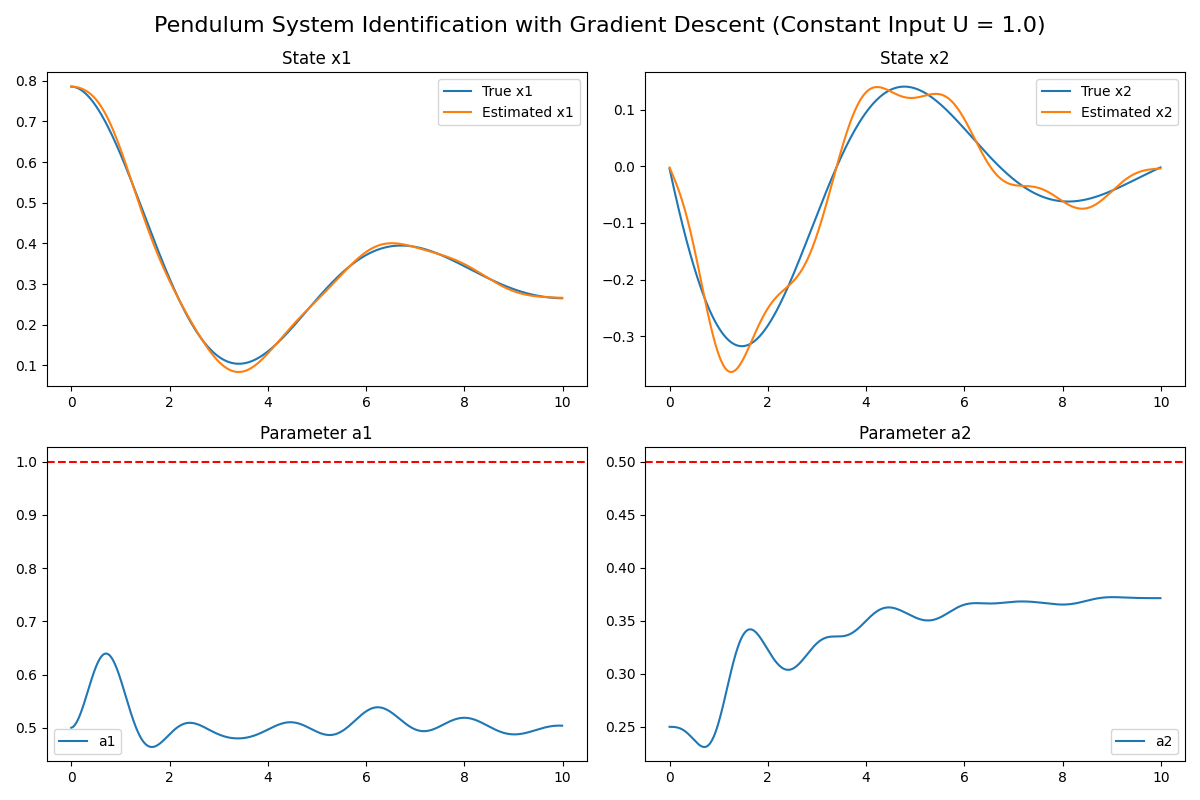
\includegraphics[width=\textwidth]{./estimation-const-unit-input.png}
    \caption{Εκτίμηση παραμέτρων με σταθερή είσοδο}
\end{figure}

Φαίνεται ότι η εκτίμηση της πρώτης παραμέτρου δεν είναι ιδιαίτερα καλή ενώ η εκτίμηση
της δεύτερης δείχνει πράγματι την τάση να συγκλίνει στην πραγματική τιμή. Ωστόσο,
η προβλεπόμενη απόκριση του συστήματος είναι πιστή στην πραγματικότητα.

\begin{figure}[h]
    \centering
    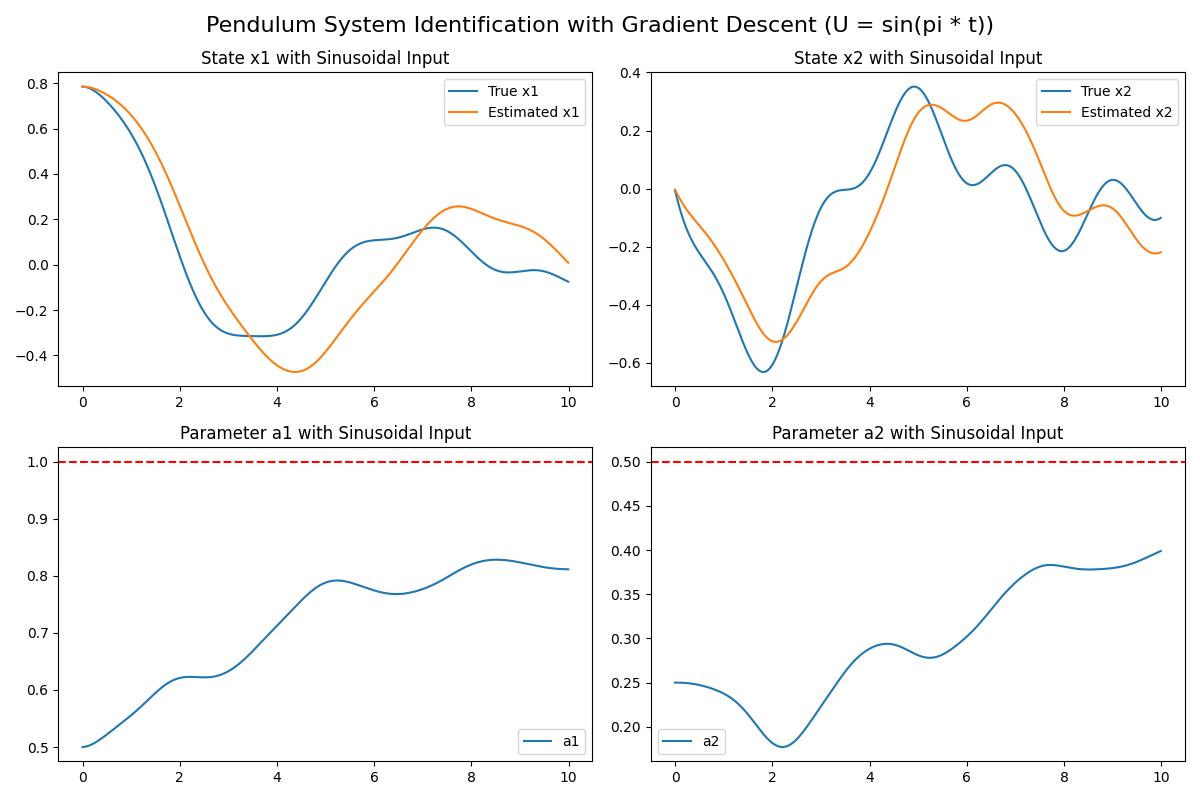
\includegraphics[width=\textwidth]{./estimation-sin-input.png}
    \caption{Εκτίμηση παραμέτρων με ημιτονοειδή είσοδο}
\end{figure}

Στην περίπτωση της ημιτονοειδούς εισόδου, φαίνεται ότι η εκτίμηση των παραμέτρων
πλησιάζει περισσότερο της πραγματικές τους τιμές, καθώς επίσης ελαττώνεται η ακρίβεια
της προβλεπόμενης απόκρισης του συστήματος.


\clearpage
\subsection{Ερώτημα}

\selectlanguage{english}
\begin{python}
from scipy.signal import square

# Function to generate a square wave
def square_wave(t, amplitude, frequency):
    return amplitude * square(2 * np.pi * frequency * t)

# Simulation parameters for square wave input
sw_frequency = 0.5  # frequency of the square wave
sw_amplitude = 1.0  # amplitude of the square wave

# Reset initial guesses for the parameters
a1, a2, b = 0.5, 0.25, 0.15  # reset to initial guesses

# Reset initial state
x = np.array(x0)
x_hat = np.array(x0)  # reset initial estimate

# Reset storage for data
x_storage = np.zeros((len(t), 2))
x_hat_storage = np.zeros((len(t), 2))
a1_storage = np.zeros(len(t))
a2_storage = np.zeros(len(t))
b_storage = np.zeros(len(t))

# Simulation loop with square wave input
for i in range(len(t)):
    # Square wave input
    u = square_wave(t[i], sw_amplitude, sw_frequency)

    # System dynamics
    x_dot = pendulum_dynamics(x, true_a1, true_a2, true_b, u)
    x = x + x_dot * dt

    # Estimated dynamics
    x_hat_dot = pendulum_dynamics(x_hat, a1, a2, b, u)
    x_hat = x_hat + x_hat_dot * dt

    # Parameter update
    a1, a2, b = update_parameters(x, x_hat, a1, a2, b, u, learning_rate)

    # Store data
    x_storage[i] = x
    x_hat_storage[i] = x_hat
    a1_storage[i] = a1
    a2_storage[i] = a2
    b_storage[i] = b
\end{python}
\selectlanguage{greek}

Τα αποτελέσματα της προσομοίωσης φαίνονται στην εικόνα που ακολουθεί.

\begin{figure}[h]
    \centering
    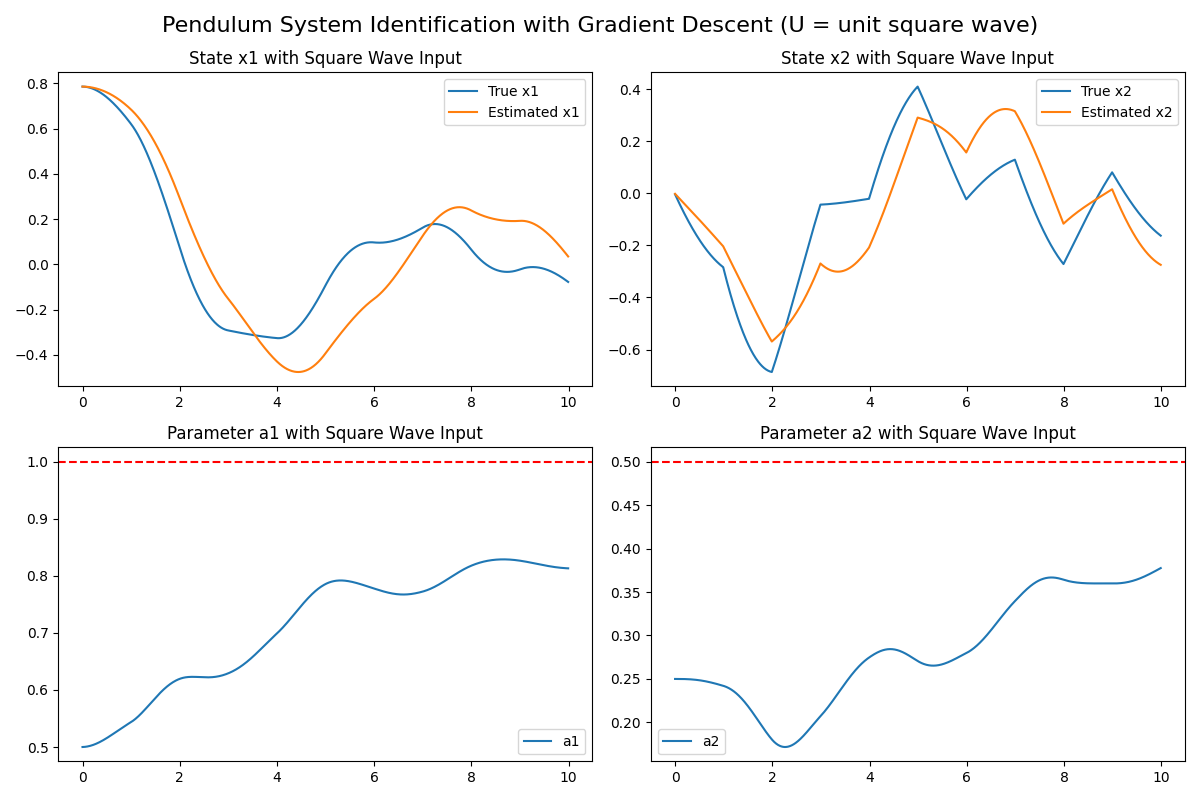
\includegraphics[width=\textwidth]{./estimation-square-wave-input.png}
    \caption{Εκτίμηση παραμέτρων με τετραγωνική είσοδο}
\end{figure}

Ομοίως με την περίπτωση της ημιτονοειδούς εισόδου, η εκτίμηση των παραμέτρων
πλησιάζει περισσότερο της πραγματικές τους τιμές, καθώς επίσης ελαττώνεται η ακρίβεια
της προβλεπόμενης απόκρισης του συστήματος. Σημειώνεται ότι η απόκριση του συστήματος
δεν είναι ομαλή, λόγω του χαρακτήρα της τετραγωνικής εισόδου, ωστόσο η εκτίμηση της
δυναμικής του συστήματος είναι αρκετά καλή.

\end{document}
